\documentclass[letterpaper]{article}
\usepackage[utf8]{inputenc}
\usepackage[spanish]{babel}
\usepackage{amssymb, amsmath}
\usepackage{stackengine}
\usepackage{graphicx}
\usepackage{lipsum}
\usepackage{dsfont}
\usepackage[margin=1.5cm,
vmargin={1.5cm,0.7cm},
includefoot]{geometry}
\usepackage{setspace}
\usepackage{subcaption}
\usepackage{tocloft}
\usepackage{upgreek}
\usepackage{amsthm}
\usepackage{graphicx}
\usepackage{paralist}
\usepackage{fancyhdr}
\usepackage{lmodern}
\usepackage{tcolorbox}
\usepackage{color}
\usepackage{tikz}
\usepackage{wasysym}
\usepackage{textgreek, marvosym}
\tcbuselibrary{skins,breakable}
\pagestyle{fancy}

\renewcommand{\headrulewidth}{0.4pt}
\renewcommand{\footrulewidth}{0.4pt}

\renewcommand{\d}{\partial}

\providecommand{\abs}[1]{\left|#1\right|}
\providecommand{\norm}[1]{\left|\left|#1\right|\right|}														  
\providecommand{\pint}[1]{\langle#1\rangle}														  
\newcommand{\V}{\mathds{V}}

\newcommand{\W}{\mathds{W}}

\newcommand{\F}{\mathds{F}}

\newcommand{\tq}{ \quad \cdot  \backepsilon \cdot \quad }

\newcommand{\ld}{\lim\limits_{x \to 0^{+}}}

\newcommand{\li}{\lim\limits_{x \to 0^{-}}}

\newcommand{\la}{\lim\limits_{x \to a}}

\renewcommand{\l}{\ell}

\newcommand{\R}{\mathds{R}}

\newcommand{\Po}{\mathds{P}_2(\mathds{R})}

\renewcommand{\*}{\cdot}

\newcommand{\Iden}{\begin{pmatrix}
		1 & 0 & 0\\
		0 & 1 & 0\\
		0 & 0 & 1 
\end{pmatrix}}
\newcommand{\T}{\begin{pmatrix}
		1 & 3 & 9 \\
		1 & 3 & 4 \\
		0 & 0 & 2 
\end{pmatrix} }

\makeatletter
\renewcommand*\env@matrix[1][\arraystretch]{%
	\edef\arraystretch{#1}%
	\hskip -\arraycolsep
	\let\@ifnextchar\new@ifnextchar
	\array{*\c@MaxMatrixCols c}}
\makeatother

\newtheorem{theorem}{Teorema}[section]
\theoremstyle{definition}
\newtheorem{definition}{Definición}


\begin{document}
	
	\setlength{\unitlength}{1cm}
	\thispagestyle{empty}
	\begin{picture}(19,3)
	\put(-0.5,1.2){
\includegraphics[scale=.20]{img/unam1.png}}
	\put(16,1){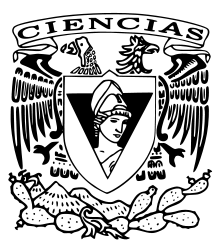
\includegraphics[scale=.29]{img/fciencias1.png}}
	\end{picture}
	
	\begin{center}
		\vspace{-114pt}
		\textbf{\large Matemáticas para las Ciencias II}\\
		\textbf{ Semestre 2020-2}\\
		Prof. Pedro Porras Flores\\
		Ayud. Irving Hernández Rosas \\
		\textbf{Proyecto III}\\[0.2cm]
		Kevin Ariel Merino Peña\footnote{Número de cuenta 317031326}\\ [0.2cm]
	\end{center}
	\vspace{-10pt}
	\rule{19cm}{0.3mm}
	
\noindent Realice los siguientes ejercicios, escribiendo el procedimiento claramente. Y recuerden que estos proyectos se entregan de manera individual en la plataforma de google classroom.\\




% -----------------------------------------------------
% Problema uno
% -----------------------------------------------------

\noindent1.  Calcule la matriz de la derivadas parciales de: 

\begin{definition}
	Ses $ U $ un conjunto abierto en $ \R^n $ y sea $ f:U\subset \R^n \to \R^m $. Se dice que $ f $ es diferenciable en $ \vec{x_0} \in U$  si todas las derivadas parciales existen y además si el siguiente límite existe: 
	\[ \lim\limits_{\vec{x} \to \vec{x_0} } \dfrac{\norm{f(\vec{x}) - f(\vec{x_0}) - T(\vec{x} - \vec{x_0})} }{\norm{\vec{x} - \vec{x_0}}} =0 \]
	Donde $ T= Df(\vec{x_0}) \in M_{mxn} $ cuyos elementos son $ \dfrac{\partial f_i}{\partial x_j} $ con $ 1 \leq i \leq m $ y $ 1 \leq j \leq n $. Esto es
	\begin{align*}
		Df(\vec{x_0}) &= \begin{pmatrix}[2.5]
		\dfrac{\partial f_1}{\d x_1 } & \dfrac{\d f_1}{\d x_2} & \dots & \dfrac{\d f_1}{\d x_n}\\
		\dfrac{\partial f_2}{\d x_1 } & \dfrac{\d f_2}{\d x_2} & \dots & \dfrac{\d f_2}{\d x_n}\\
		\vdots & & \ddots & \\
		\dfrac{\partial f_m}{\d x_1 } & \dfrac{\d f_m}{\d x_2} & \dots & \dfrac{\d f_m}{\d x_n}\\
		\end{pmatrix}
	\end{align*}
	Es llamada matriz de las derivadas parciales o Matriz Jacobiana
\end{definition}

\noindent a) $f: \mathbb{R}^2  \longrightarrow \mathbb{R}^2$, tal que $f(x,y) = (e^x,\sin(xy))$
\begin{align*}
	Df(\vec{x_0}) &= \begin{pmatrix}[2.5]
	\dfrac{\d e^x}{\d x} & \dfrac{\d e^x}{\d y}\\
	\dfrac{\d \sin(xy)}{\d x} & \dfrac{\d \sin(xy)}{\d y}\\
	\end{pmatrix} && \text{Por definición de la matriz Jacobiana}\\
	Df(\vec{x_0}) &= \begin{pmatrix}[2.5]
	e^x & \dfrac{\d e^x}{\d y}\\
	\dfrac{\d \sin(xy)}{\d x} & \dfrac{\d \sin(xy)}{\d y}\\
	\end{pmatrix} && \text{La derivada de $ e^x $ es la función misma (cálculo I)}\\
	Df(\vec{x_0}) &= \begin{pmatrix}[2]
	e^x & 0\\
	\dfrac{\d \sin(xy)}{\d x} & \dfrac{\d \sin(xy)}{\d y}\\
	\end{pmatrix} && \text{Puesto que $ x $ figura como constante}\\
	Df(\vec{x_0}) &= \begin{pmatrix}[2]
	e^x & 0\\
	y\dfrac{\d \sin(xy)}{\d x} & x\dfrac{\d \sin(xy)}{\d y}\\
	\end{pmatrix} && \text{Por regla de la cadena}\\
	Df(\vec{x_0}) &= \begin{pmatrix}[1.5]
	e^x & 0\\
	y\cos(xy) &x\cos(xy)\\
	\end{pmatrix} && \text{Efectuando las derivadas parciales}\\
\end{align*}


\noindent b) $f: \mathbb{R}^2  \longrightarrow \mathbb{R}^3$, tal que $f(x,y) = (xe^y + \cos(y), x, x + e^y)$

\begin{align*}
	Df(\vec{x_0}) &= \begin{pmatrix}[2.5]
	\dfrac{\d}{\d x} (xe^y + \cos(y)) & \dfrac{\d}{\d y} (xe^y + \cos(y))\\
	\dfrac{\d}{\d x} x & \dfrac{\d}{\d y} x\\
	\dfrac{\d}{\d x} (x + e^y) & \dfrac{\d}{\d y}( x + e^y)\\
	\end{pmatrix} &&\text{Por definición de matriz de derivadas parciales}\\
	Df(\vec{x_0}) &= \begin{pmatrix}[2.5]
	  e^y\dfrac{\d}{\d x} x + \dfrac{\d}{\d x}\cos(y) & x\dfrac{\d}{\d y} e^y + \dfrac{\d}{\d y}\cos(y)\\
	\dfrac{\d}{\d x} x & \dfrac{\d}{\d y} x\\
	\dfrac{\d}{\d x} x + \dfrac{\d}{\d x}e^y & \dfrac{\d}{\d y} x + \dfrac{\d}{\d y}e^y\\
	\end{pmatrix} &&\text{Empleamos que la derivada es lineal, abre sumas y saca escalares}\\
	Df(\vec{x_0}) &= \begin{pmatrix}[1.5]
	e^y & x e^y - \sin(y)\\
	1 & 0\\
	1 & e^y\\
	\end{pmatrix} &&\text{Operando las derivadas}
\end{align*}

\noindent c) $f: \mathbb{R}^3  \longrightarrow \mathbb{R}^2$, tal que $f(x,y,z) = (x + e^z + y, xy^2)$
\begin{align*}
	Df(\vec{x_0}) &= \begin{pmatrix}[2.5]
	\dfrac{\d}{\d x} (x + e^z + y) & \dfrac{\d}{\d y} (x + e^z + y) & \dfrac{\d}{\d z} (x + e^z + y) \\
	\dfrac{\d}{\d x} (xy^2) & \dfrac{\d}{\d y}( xy^2) & \dfrac{\d}{\d z} (xy^2) \\
	\end{pmatrix} && \text{Definición de matriz de derivadas parciales}\\
	Df(\vec{x_0}) &= \begin{pmatrix}[2.5]
	\dfrac{\d}{\d x} x + \dfrac{\d}{\d x} e^z + \dfrac{\d}{\d x} y & \dfrac{\d}{\d y} x + \dfrac{\d}{\d y} e^z +\dfrac{\d}{\d y} y & \dfrac{\d}{\d z} x + \dfrac{\d}{\d z} e^z + \dfrac{\d}{\d z}y \\
	y^2\dfrac{\d}{\d x} x & x\dfrac{\d}{\d y}y^2 & \dfrac{\d}{\d z} (xy^2) \\
	\end{pmatrix} && \text{Usamos que la derivada es un operador lineal}\\
	Df(\vec{x_0}) &= \begin{pmatrix}[1.5]
	1& 1 & e^z \\
	y^2 & 2xy & 0 
	\end{pmatrix} && \text{Efectuando las derivadas parciales}
\end{align*}

\noindent d) $f: \mathbb{R}^3  \longrightarrow \mathbb{R}^2$, tal que $f(x,y) = (xye^{xy}, x\sin(y), 5xy^2)$
\begin{align*}
	Df(\vec{x_0}) &= \begin{pmatrix}[2.5]
	\dfrac{\d }{\d x} xye^{xy}  & \dfrac{\d }{\d y} xye^{xy} \\
	\dfrac{\d }{\d x} x\sin(y) & \dfrac{\d }{\d y} x\sin(y) \\
	\dfrac{\d }{\d x}  5xy^2 & \dfrac{\d }{\d y}  5xy^2
	\end{pmatrix} && \text{Definición de matriz de derivadas parciales}\\
	Df(\vec{x_0}) &= \begin{pmatrix}[2.5]
	y\dfrac{\d }{\d x} e^{xy}x  & x\dfrac{\d }{\d y} ye^{xy}\\
	\sin(y)\dfrac{\d }{\d x} x & x\dfrac{\d }{\d y} \sin(y) \\
	5y^2\dfrac{\d }{\d x}  x & 5x\dfrac{\d }{\d y}  y^2 
	\end{pmatrix} && \text{Empleando que la derivada es operador lineal}
\end{align*}
\begin{align*}
	Df(\vec{x_0}) &= \begin{pmatrix}[2.5]
	y(e^{yx} + xye^{xy})  & x(e^{xy} + xye^{xy}) \\
	\sin(y) & x\cos(y)\\
	5y^2 & 10xy
	\end{pmatrix} && \text{Operando las dervidas parciales}
\end{align*}

\noindent 2.  Sea $f(x,y) = xe^{y^2} - ye^{x^2}$\\

\begin{definition}[Plano tangente]
	Sea $ f: \R^2 \to \R $ una función diferenciable en $ \vec{x_0} = (x_0, y_0) $. El plano tangente en $ \R^3 $ definido por la ecuación
	\[ z = f(x_0, y_0) + \left[ \dfrac{\d f}{\d x} (x_0, y_0) \right](x - x_0) + \left[ \dfrac{\d f}{\d y}(x_0, y_0) \right](y-y_0) \]
	Es llamado plano tangente a la gráfica de $ f $ en el punto $ (x_0,y_0) $
\end{definition}
\noindent a) Encuentre el plano tangente a la gráfica de $f$ en $(1, 2)$

\begin{align*}
	z &= f(x_0, y_0) + \left[ \dfrac{\d f}{\d x} (x_0, y_0) \right](x - x_0) + \left[ \dfrac{\d f}{\d y}(x_0, y_0) \right](y-y_0) && \text{Planteando la ecuación}\\
	z &= f(1, 2) + \left[ \dfrac{\d f}{\d x} (1, 2) \right](x - 1) + \left[ \dfrac{\d f}{\d y}(1, 2) \right](y-2) && \text{Observemos que } x_0 = 1, y_0 = 2\\
	z &= (e^4-2e) + \left[ \dfrac{\d f}{\d x} (1, 2) \right](x - 1) + \left[ \dfrac{\d f}{\d y}(1, 2) \right](y-2) && \text{Evaluando } f(1,2)\\
	z &= (e^4-2e) + \left[ \dfrac{\d }{\d x} (xe^{y^2} - ye^{x^2}) \right]\Bigr|_{\substack{(1, 2)}} (x - 1) + \left[ \dfrac{\d }{\d y}(xe^{y^2} - ye^{x^2}) \right]\Big|_{\substack{(1, 2)}}(y-2) && \text{Cambiando regla de correspondencia de } f\\
	z &= (e^4-2e) + \left[ e^{y^2} - 2e^{x^2} xy \right]\Bigr|_{\substack{(1, 2)}} (x - 1) + \left[ 2xe^{y^2} y-e^{x^2} \right]\Big|_{\substack{(1, 2)}}(y-2) && \text{Con las parciales de } f\\
	z &= (e^4-2e) + (-4e + e^4) (x - 1) + (4e^4-e)(y-2) && \text{Evaluando en el punto dado} \\
	z &= e^4-2e + -4ex + e^4x+ 4e - e^4  + 4e^4y - ey -8e^4 +2e  && \text{Por distributividad }\\
	z &= (e^4-4e)x +(4e^4-e)y-8e^4+4e && \text{Agrupando términos semejantes }
\end{align*}

\noindent b) ¿Qué punto sobre la superficie $z = x^2 -y^2$, tiene un plano tangente paralelo al plano tangente encontrado en la primer parte?\\

Notemos que $ \vec{n} = (e^4-4e,4e^4-e,-1) $ es un vector normal en el plano del ejericicio anterior.

Empleando $ z = x^2 - y^2 $ definamos una nueva función $ g: \R^2 \to \R $ como $ g(x,y) = x^2 - y^2 $.

Por otra parte, veamos que en $ (x_0,y_0) $ la normal al plano tangente en el punto $ (x_0,y_0,g(x_0,y_0)) $ está definido como 
\[ \vec{m} = \left( \dfrac{\d g}{\d x}(x_0, y_0), \dfrac{\d g}{\d y}(x_0,y_0),-1 \right) \]
Esto último significa que nos fijaremos en los puntos $ (x_0,y_0) $ que cumplan \[ \vec{m} = \alpha\vec{n} \] con $ \alpha \in \R $, ahora obtengamos las derivadas parciales 
\begin{align*}
	\dfrac{\d g}{\d x}(x_0, y_0) &= \alpha(e^4-4e) && \text{Por  que estamos buscando puntos de esta forma}\\
	\dfrac{\d g}{\d y}(x_0, y_0) &= \alpha(4e^4-e) && \text{ }\\
\end{align*}
\begin{align*}
	\dfrac{\d g}{\d x}(x_0, y_0) &= (x^2)' && \text{ Por definición de }g\\
	\dfrac{\d g}{\d y}(x_0, y_0) &= (-y^2)' && \text{ }\\
	\dfrac{\d g}{\d x}(x_0, y_0) &= 2x && \text{Aplicando la derivada }\\
	\dfrac{\d g}{\d y}(x_0, y_0) &= -2y && \text{ }
\end{align*}
Así, los puntos $ (x_0,y_0) $ que buscamos son de la forma 
\[ (x_0,y_0) = \dfrac{\alpha}{2}(e^4-4e,e-4e^4) \iff (x_0,y_0) = \alpha(e^4-4e,e-4e^4) \]
Tomemos $ \alpha = 1 $ entonces tenemos el punto
\[ (e^4-4e,e-4e^4, -15e^2(e^6-1) ) \]

\noindent 3.  Calcule el gradiente de las siguientes funciones:\\

\begin{definition}[Gradiente]
	Sea $ f: \R^n \to \R $.
	Definimos al gradiente de $ f $ como 
	\[ \nabla f(\vec{x}) = \left( \dfrac{\d}{\d x_1}, \dfrac{\d}{\d x_2}, \dots, \dfrac{\d}{\d x_n}  \right) \]
\end{definition}
\noindent a) $f(x,y,z) = x e^{-(x^2 +y^2 +z^2)}$
\begin{align*}
	\dfrac{\d f}{\d x} &= \dfrac{\d}{\d x} (x e^{-(x^2 +y^2 +z^2)}) && \text{Planteando la derivada parcial con respecto a } x\\
	\dfrac{\d f}{\d x} &= x\dfrac{\d}{\d x} e^{-(x^2 +y^2 +z^2)} + e^{-(x^2 +y^2 +z^2)} \dfrac{\d}{\d x} x && \text{Por la derivada de productos }\\
	\dfrac{\d f}{\d x} &= x\dfrac{\d}{\d x} e^{-(x^2 +y^2 +z^2)} + e^{-(x^2 +y^2 +z^2)} && \text{Por neutro multiplicativo }\\
	\dfrac{\d f}{\d x} &= xe^{-(x^2 +y^2 +z^2)}-2x + e^{-(x^2 +y^2 +z^2)} && \text{Por la regla de la cadena }\\
	\dfrac{\d f}{\d x} &= -2x^2e^{-(x^2 +y^2 +z^2)} + e^{-(x^2 +y^2 +z^2)} && \text{Conmutantando }\\
	\dfrac{\d f}{\d x} &= -e^{-(x^2 +y^2 +z^2)}(-2x^2 +1) && \text{Factorizando  }\\
	\\
	\dfrac{\d f}{\d y} &= \dfrac{\d}{\d y}(x e^{-(x^2 +y^2 +z^2)}) && \text{Planteando la derivada parcial}\\
	\dfrac{\d f}{\d y} &= x\dfrac{\d}{\d y}e^{-(x^2 +y^2 +z^2)} && \text{Empleando que la derivada es lineal}\\
	\dfrac{\d f}{\d y} &= xe^{-(x^2 +y^2 +z^2)}-2y && \text{Por la regla de la cadena}\\
	\dfrac{\d f}{\d y} &= -2yxe^{-(x^2 +y^2 +z^2)} && \text{Conmutando el producto}\\
	\\
	\dfrac{\d f}{\d z} &= \dfrac{\d}{\d z} (x e^{-(x^2 +y^2 +z^2)}) && \text{Planteando la derivada parcial}\\
	\dfrac{\d f}{\d z} &= x\dfrac{\d}{\d z} e^{-(x^2 +y^2 +z^2)} && \text{Porque la derivada es un operador lineal}\\
	\dfrac{\d f}{\d y} &= xe^{-(x^2 +y^2 +z^2)}-2z && \text{Por la regla de la cadena}\\
	\dfrac{\d f}{\d y} &= -2zxe^{-(x^2 +y^2 +z^2)} && \text{Conmutando el podcuto}\\
\end{align*}
\begin{center}
	$ \therefore \nabla f(x,y,z) = e^{-(x^2 +y^2 +z^2)} ( -2x^2 +1, -2yx, -2zx ) $
\end{center}
\noindent b) $f(x,y,z) = \dfrac{xyz}{x^2 +y^2 +z^2}$\\
\begin{align*}
	\dfrac{\d f}{\d x} &= \dfrac{\d}{\d x} \left(\dfrac{xyz}{x^2 +y^2 +z^2}\right) && \text{Planteando la derivada parcial}\\
	\dfrac{\d f}{\d x} &= \dfrac{ (x^2+y^2+z^2)\dfrac{\d}{\d x}(xyz) - xyz\dfrac{\d}{\d x}(x^2 + y^2 + z^2) }{(x^2 + y^2 + z^2)^2} && \text{Reglas de derivada de Calculo I}\\
	\dfrac{\d f}{\d x} &= \dfrac{ (x^2+y^2+z^2)yz - xyz(2x) }{(x^2 + y^2 + z^2)^2} && \text{Derivando la parcial }\\
	\dfrac{\d f}{\d x} &= \dfrac{ -x^2yz+y^3z+yz^3 }{(x^2 + y^2 + z^2)^2}&& \text{Sumando términos semejantes }\\
	\\
	\dfrac{\d f}{\d y} &= \dfrac{\d}{\d y} \left(\dfrac{xyz}{x^2 +y^2 +z^2}\right)&&\text{Planteando la derivada parcial}\\
		\dfrac{\d f}{\d y} &= \dfrac{ (x^2+y^2+z^2)\dfrac{\d}{\d y}(xyz) - xyz\dfrac{\d}{\d y}(x^2 + y^2 + z^2) }{(x^2 + y^2 + z^2)^2} && \text{Reglas de derivada de Calculo I}\\
	\dfrac{\d f}{\d y} &= \dfrac{ (x^2+y^2+z^2)xz - xyz(2y) }{(x^2 + y^2 + z^2)^2} && \text{Derivando la parcial }\\
	\dfrac{\d f}{\d y} &= \dfrac{ x^3z-xy^2z+xz^3 }{(x^2 + y^2 + z^2)^2}&& \text{Sumando términos semejantes }\\
	\\
	\dfrac{\d f}{\d z} &= \dfrac{\d}{\d z} \left(\dfrac{xyz}{x^2 +y^2 +z^2}\right) && \text{Planteando la derivada parcial}\\
		\dfrac{\d f}{\d z} &= \dfrac{ (x^2+y^2+z^2)\dfrac{\d}{\d z}(xyz) - xyz\dfrac{\d}{\d z}(x^2 + y^2 + z^2) }{(x^2 + y^2 + z^2)^2} && \text{Reglas de derivada de Calculo I}\\
	\dfrac{\d f}{\d z} &= \dfrac{ (x^2+y^2+z^2)xy - xyz(2z) }{(x^2 + y^2 + z^2)^2} && \text{Derivando la parcial }\\
	\dfrac{\d f}{\d z} &= \dfrac{ x^3y+xy^3-xyz^2 }{(x^2 + y^2 + z^2)^2}&& \text{Sumando términos semejantes }
\end{align*}
\[ \therefore \nabla f(x,y,z) = \dfrac{1}{(x^2 + y^2 + z^2)^2} \left(  yz(-x^2+y^2+z^2), xz(x^2-y^2+z^2), xy(x^2+y^2-z^2) \right) \]

\noindent c) $f(x,y,z) = z^2e^x\cos(y)$
\begin{align*}
	\dfrac{\d f}{\d x} &= \dfrac{\d}{\d x} z^2e^x\cos(y) &&\text{Planteando la parcial}\\
	\dfrac{\d f}{\d x} &= z^2\cos(y)\dfrac{\d}{\d x} e^x &&\text{Porque la derivada es lineal y saca escalares}\\
	\dfrac{\d f}{\d x} &= z^2\cos(y)e^x &&\text{Por nuestro curso de Cálculo I}\\
	\\
	\dfrac{\d f}{\d y} &= \dfrac{\d}{\d x} z^2e^x\cos(y) &&\text{Planteando la parcial}\\
	\dfrac{\d f}{\d y} &= z^2e^x(-\sin(y)) &&\text{Por derivadas de trigonométricas}\\
	\dfrac{\d f}{\d y} &= -z^2e^x\sin(y) &&\text{Asociando }
\end{align*}
\begin{align*}
		\dfrac{\d f}{\d z} &= \dfrac{\d}{\d z} z^2e^x\cos(y) &&\text{Planteando la parcial}\\
	\dfrac{\d f}{\d z} &= e^x\cos(y)2z &&\text{Por reglas de la derivada de exponentes}
\end{align*}
\[ \therefore \nabla f(x,y,z) = ze^x(z\cos(y), -z\sin(y), 2\cos(y)) \]



\noindent 4. Haga un bosquejo de las curvas que son las imágenes de las siguientes trayectorias:\\


\noindent a) $\vec{\gamma}(t) = (\sin(t), 4\cos(t))$, donde $0 \leq t \leq 2\pi$\\
Sea sea $ t \in [0,2\pi] $, tomemos un ligero cambio de variable y así tenemos que:

\begin{align*}
x &= \sin(x)  \quad y= 4\cos(t)\\
\dfrac{x^2 }{1^2}+ \dfrac{y^2}{4^2} &= 	\sin^2t + \cos^2t = 1
\end{align*}
y hace un par de semanas justo revisamos en clase que este tipo de cónicas son elipses, además podemos decir dónde se encuentran sus vértices, que es en $ (-1,0),(1,0),(0,4),(0,-4) $\\

\begin{figure}[h!]
	\centering
	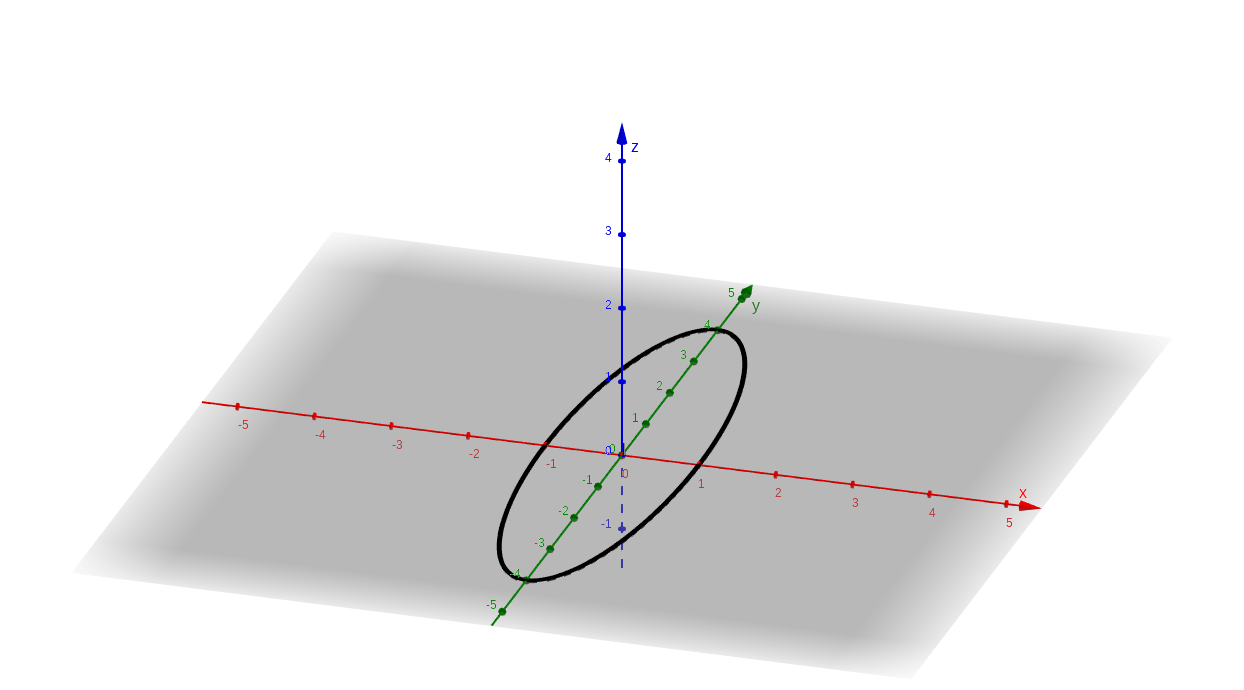
\includegraphics[width=\textwidth]{img/proyecto4_5.png}
	\caption{Curva trazada por $ \vec{\gamma}(t) = (\sin(t), 4\cos(t))$}
\end{figure}

\noindent b) $\vec{\gamma}(t) = (2\sin(t), 4\cos(t))$, donde $0 \leq t \leq 2\pi$\\
Sea $ t \in [0,\pi] $, tomemos un cambio de variables como $ x = 2\sin(t), \quad y= 4\cos(t) $ tenemos que:
\[ \dfrac{x^2}{2^2} + \dfrac{y^2}{4^2} = 1 \quad\quad \sin^2(t) + \cos^2(t) = 1  \]
Además de esta elipse podemos decir que sus vértices se encuentran en $ (\pm 2,0), (0,\pm 4) $

\begin{figure}[h!]
	\centering
		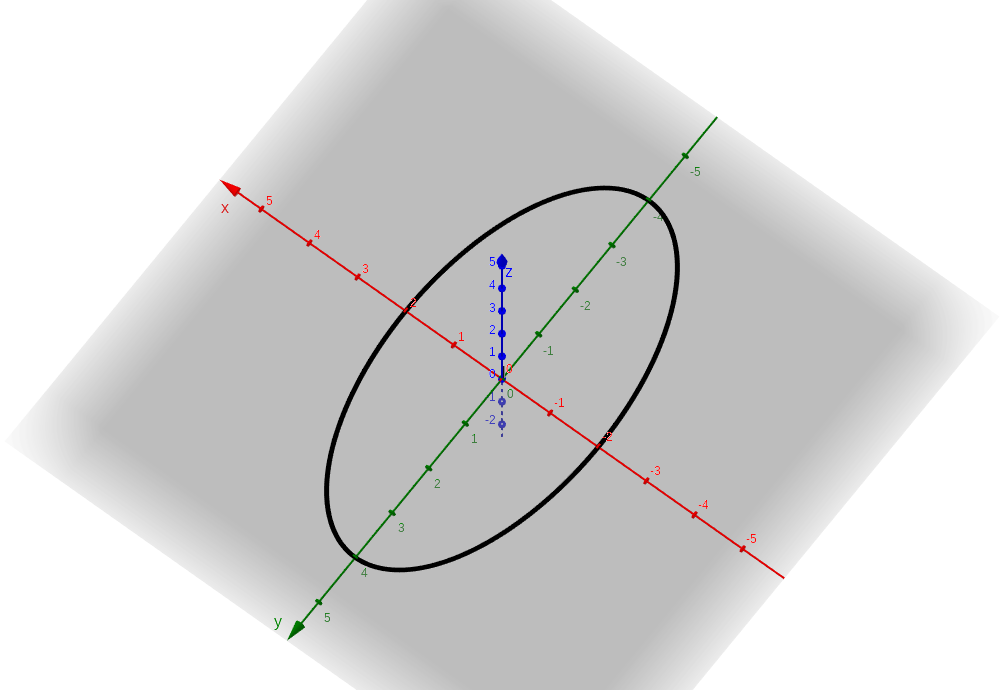
\includegraphics[width=0.5\textwidth]{img/Proyecto4_6.png}
		\caption{Curva trazada por $ \vec{\gamma}(t)= (2\sin(t), 4\cos(t)) $}
\end{figure}

\newpage
\noindent c) $\vec{\gamma}(t) = (t\sin(t), t\cos(t), t)$, donde $ -4\pi \leq t \leq 4\pi$\\

\begin{figure}[h!]
	\centering
	\begin{subfigure}[b]{0.3\linewidth}
	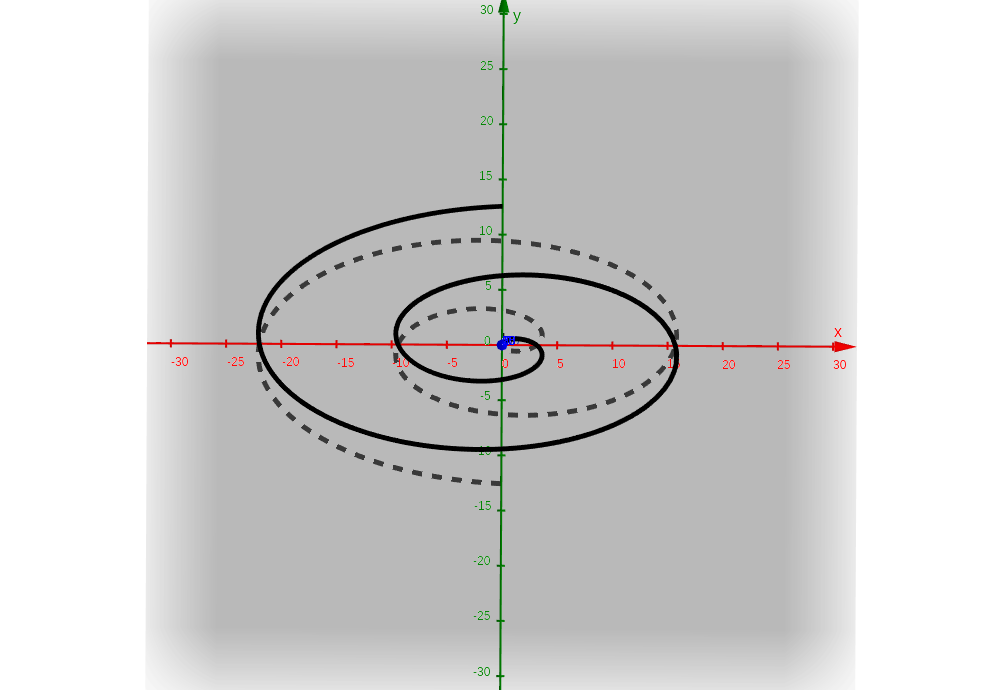
\includegraphics[width=\textwidth]{img/Proyecto4_7.png}
	\caption{Vista desde la perspectiva con el plano $ xy $}
\end{subfigure}
\begin{subfigure}[b]{0.3\linewidth}
	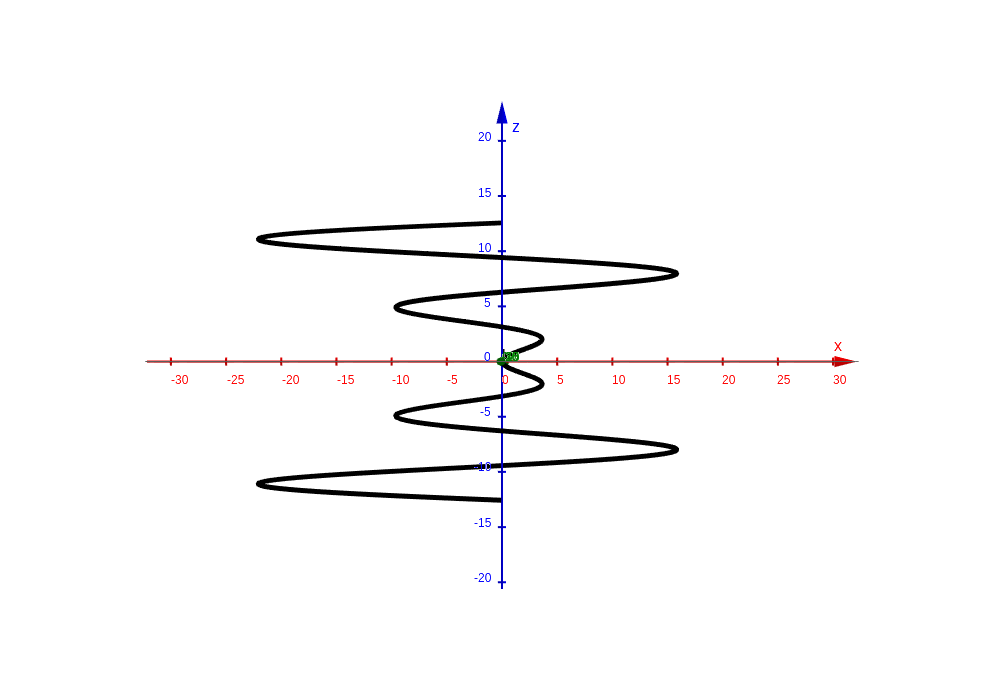
\includegraphics[width=\textwidth]{img/Proyecto4_8.png}
	\caption{Desde el plano $ zx $}
\end{subfigure}
\begin{subfigure}[b]{0.3\linewidth}
	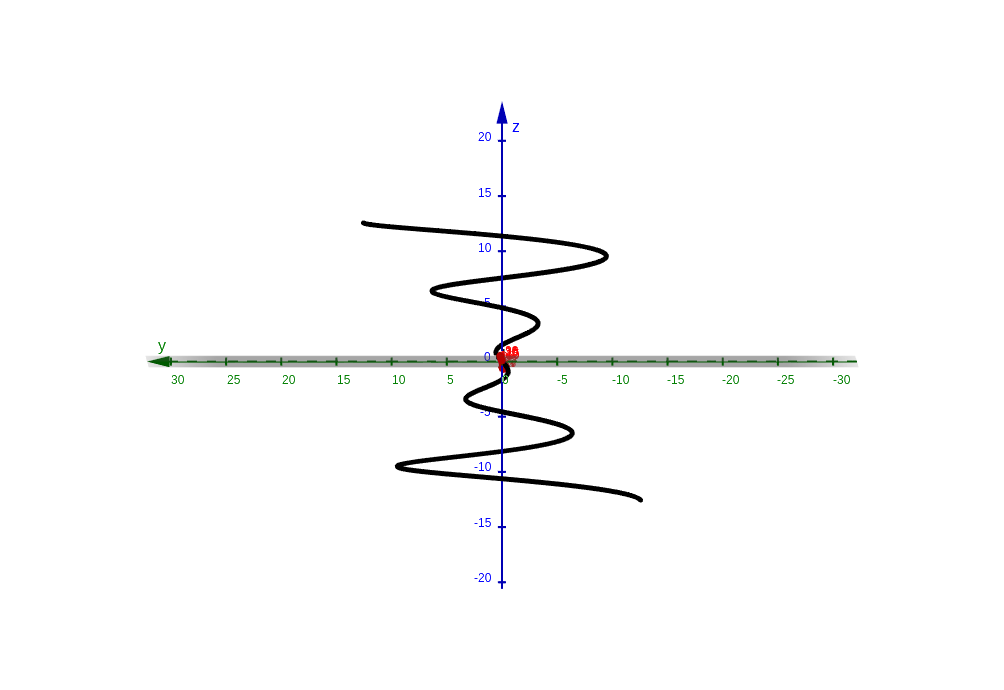
\includegraphics[width=\textwidth]{img/Proyecto4_9.png}
	\caption{Vista desde el plano $ zy $}
\end{subfigure}
\begin{subfigure}[b]{0.5\linewidth}
	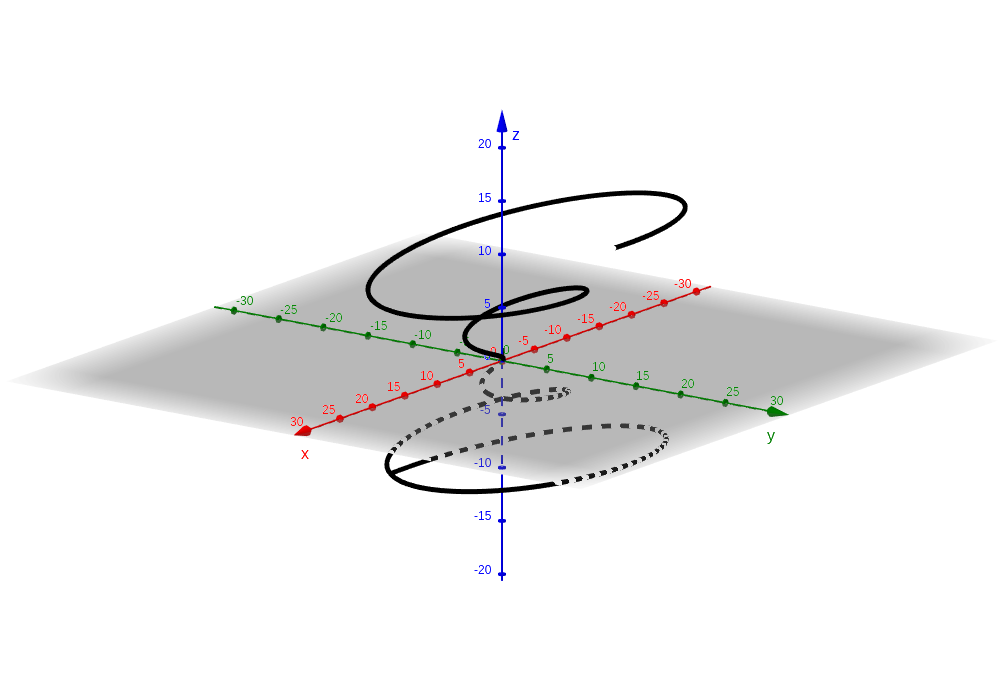
\includegraphics[width=\textwidth]{img/Proyecto4_10.png}
	\caption{Vista tridimensional en el espacio $ \R^3 $}
\end{subfigure}
	\caption{Curva trazada por $ \vec{\gamma}(t)= (t\sin(t), t\cos(t), t)$}
\end{figure}
Sobre esta trayectoria podemos decir que tiene forma de hélice, al menos porque así se define en el ejercicio 5 y por que vimos un ejemplo en clase, además se ve claramente que el radio de la hélice es la misma variable $ t $ y qe la distancia entre los lazos de dicha hélice es también $ t $ por lo que, con la herramienta adecuada podríamos describir su curvatura (pero no es el caso). En cada uno de los lados se puede ver cómo parece la gráfica de $ f(x) = x\cos(x)$ lo mismo con el seno.



\newpage
\noindent 5. El vector de posición para una partícula que se mueve sobre una hélice es: $$\vec{\gamma}(t) = (\sin(t), \cos(t), t^2)$$
\begin{figure}[h]
	\centering
	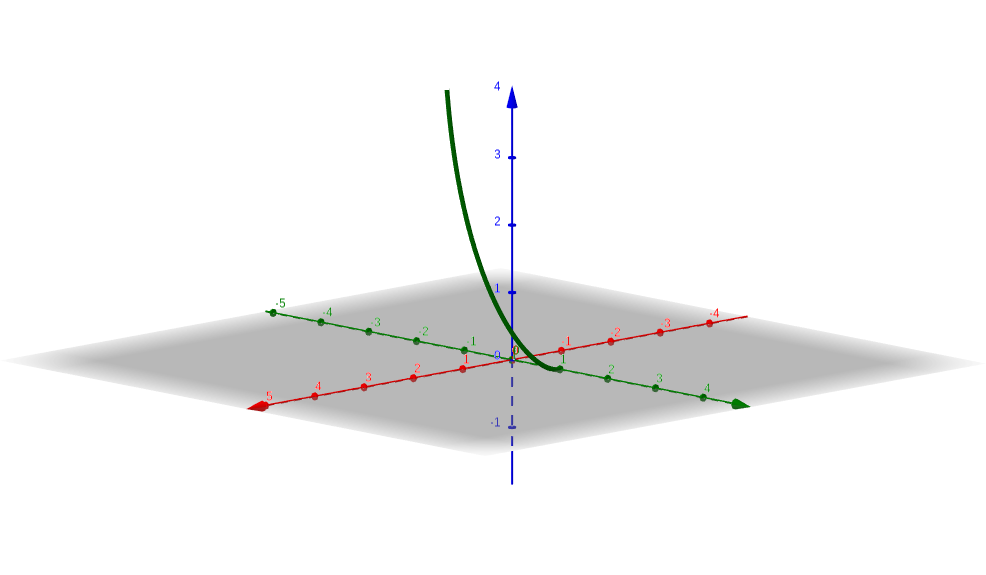
\includegraphics[width=0.8\textwidth]{img/Proyecto4.png}
	\caption{Curva trazada por $ \vec{\gamma} $}
\end{figure}
\begin{definition}[Vector velocidad]
	Si $ \vec{\gamma} $ es una trayectoria  es diferenciable, decimos que $ \vec{\gamma} $ es una trayectoria diferenciable. El vector velocidad de $ \vec{\gamma} $ en el tiempo $ t $ es definido por: \[ \vec{\gamma'} = \lim\limits_{h \to 0} \dfrac{\vec{\gamma}(t + h) - \vec{\gamma}(t)}{h} \]
	Normalmente se dibuja el vector $ \vec{\gamma'}(t) $ con la cola en el punto $ \vec{\gamma}(t) $. Si $\vec{\gamma}(t) = (x(t),y(t)) $, en $ \R^2 $, entonces:
	\[ \vec{\gamma'}(t) = (x'(t), y'(t)) = x'(t)\hat{i} + y'(t)\hat{j} \] y si \[ \vec{\gamma'}(t) = (x'(t), y'(t), z'(t) = x'(t)\hat{i} + y'(t)\hat{j} + z'(t)\hat{k} \]
\end{definition}
\begin{definition}[Rapidez]
	La rapidez de la trayectoria $ \vec{\gamma}(t) $ es $ s = \norm{\vec{\gamma'}(t)} $, es decir la longitud del vector velocidad
\end{definition}
\begin{definition}[Vector tangente]
	La velocidad $ \vec{\gamma'}(t) $ es una recta tangente a la trayectoria $ \vec{\gamma}(t) $ en el tiempo $ t $ si $ C $ es una curva trazada por $ \vec{\gamma}(t) $  si $ \vec{\gamma'}(t) \neq 0 \qquad \forall t \in $ Dominio de $ \vec{\gamma} $, entonces $ \vec{\gamma'}(t) $ es un vector tangente a la curva $ C $ en el punto $ \vec{\gamma'}(t) $
\end{definition}

\noindent a) Encuentre la rapidez de la partícula en el tiempo  $t_0 = 4\pi$\\
Para ello, primero hallemos el vector velocidad 
\begin{align*}
	\vec{\gamma'}(t_0) &= (\sin'(t) , \cos'(t), (t^2)') && \text{Por definición de velocidad}\\
	\vec{\gamma'}(t_0) &= (\cos(t), - \sin(t), 2t) && \text{Aplicando la derivada}\\
	\vec{\gamma'}(4\pi) &= (\cos(4\pi), - \sin(4\pi), 2\*4\pi) && \text{Sustituyendo el valor de }t_0\\
	\vec{\gamma'}(4\pi) &= (\cos( 0 + 2\*2\*\pi), - \sin(4\pi), 8\pi) && \text{Multiplicando escalares}
	\end{align*}
\begin{align*}
	\vec{\gamma'}(4\pi) &= (\cos(0), - \sin(4\pi), 8\pi) && \text{De cálculo I tenemos que } \cos(\alpha + 2\pi k) = \cos(\alpha)\\
	\vec{\gamma'}(4\pi) &= (\cos(0), - \sin( 0 + 2\*2\*\pi), 8\pi) && \text{Reacomodando el valor de } \sin\\
	\vec{\gamma'}(4\pi) &= (1, -\sin(0), 8\pi) && \text{De cálculo I tenemos que } \sin(\alpha + 2\pi k) = \sin(\alpha)\\
	\vec{\gamma'}(4\pi) &= (1,0, 8\pi) && \text{Finalmente obtenemos }\\
	\norm{\vec{\gamma'}(4\pi)} &= \sqrt{1^2 + 0^2 + (8\pi)^2} && \text{Por definición de norma }\\
	\norm{\vec{\gamma'}(4\pi)} &= \sqrt{1+ 8^2\pi^2} && \text{Propiedades de los exponentes }\\
	\norm{\vec{\gamma'}(4\pi)} &= \sqrt{1+ 64\pi^2} && \text{Elevando al cuadrado } 8\\
	3 &< \pi && \text{Por definición de }\pi \\
	24 &< 8\pi && \text{Por propiedades de }< \\
	24 &< \sqrt{8^2\pi^2} && \text{Pues  }8^2\pi^2 > 0 \\
	24 &< \sqrt{8^2\pi^2} < \sqrt{1 +8^2\pi^2} && \text{Ya que al menos distan una unidad  }\\
	24 &< \sqrt{1 +8^2\pi^2} && \text{Transitividad de la desigualdad }\\
	1 +8^2\pi^2 &< 676 && \text{Por curso de cálculo I} \\
	\sqrt{1 +8^2\pi^2} &< \sqrt{676} && \text{La raíz cuadrada es continua} \\
	\sqrt{1 +8^2\pi^2} &< 26 && \text{Por el valor de dicha raíz} \\
	24 &< \sqrt{1 +8^2\pi^2} < 26 && \text{Por transitividad } \\
	\norm{\vec{\gamma'}(4\pi)} &\approx 25.1526 && \text{Aproximando el resultado }
\end{align*}

\begin{figure}[h!]
	\centering
	\begin{subfigure}[b]{0.5\linewidth}
		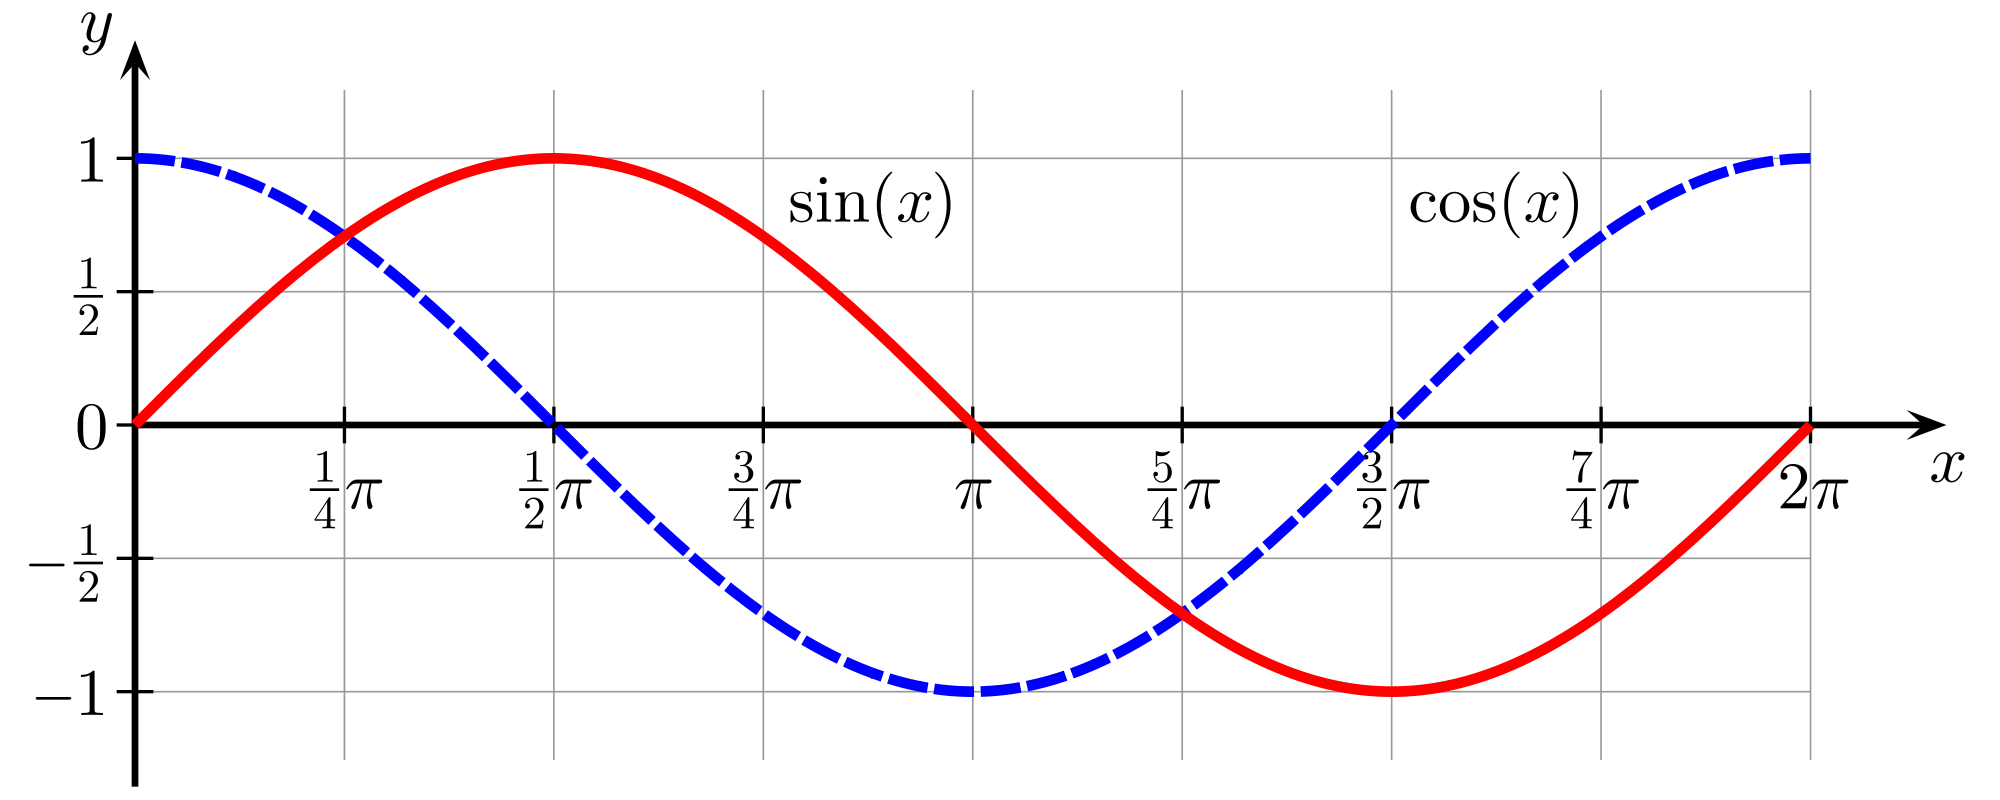
\includegraphics[width=0.9\textwidth]{img/trigo.png}
		\caption{Recordemos las gráicas de $ \sin(x),  \cos(x)$}
	\end{subfigure}
\begin{subfigure}[b]{0.85\linewidth}
	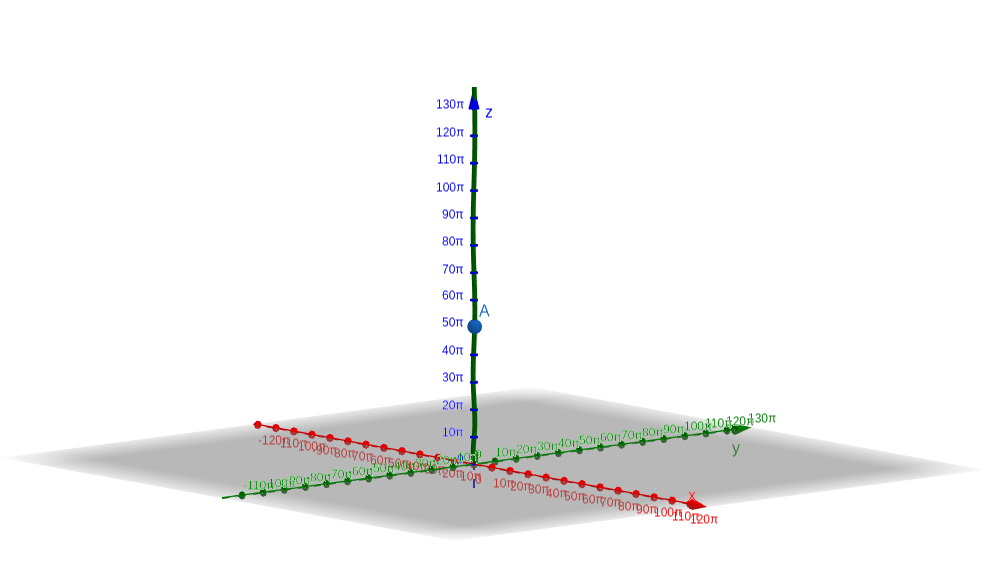
\includegraphics[width=0.9\textwidth]{img/Proyecto4_1.png}
	\caption{Localización del punto A que es $ \vec{\gamma}(4\pi) $}
\end{subfigure}
\end{figure}
\noindent b) ¿Es $\vec{\gamma}$ es ortogonal a  $\vec{\gamma'}$?
\begin{definition}[Vector ortogonal]
	Sean $\vec{x}, \vec{y} \in \V  $ decimos que $ \vec{x} $ es ortogonal a $ \vec{y} $ si y sólo si $ \pint{\vec{x},\vec{y}} = 0 $
\end{definition}
\[\begin{array}{rlc}
\vec{\gamma}(t) &= (\sin(t), \cos(t), t^2)  &\text{Recordatorio}\\
\vec{\gamma'}(t) &= (\cos(t) - \sin(t), 2t) &\text{Recordatorio}
\end{array}
 \]
 \begin{align*}
 	\pint{\vec{\gamma}, \vec{\gamma'}} & = \pint{(\sin(t), \cos(t), t^2), (\cos(t) - \sin(t), 2t)} && \text{Por recordatorio anterior}\\
 	\pint{\vec{\gamma}, \vec{\gamma'}} & = \sin(t)\* \cos(t) + \cos(t)\*(-\sin(t)) + 2t\*t^2 && \text{Por definición de producto escalar}\\
 	\pint{\vec{\gamma}, \vec{\gamma'}} & = \sin(t)\cos(t) -\sin(t)\cos(t) + 2t^3 && \text{Multiplicando términos semejantes}\\
 	\pint{\vec{\gamma}, \vec{\gamma'}} & = 2t^3 && \text{Existencia del inverso aditivo en }\R \\
 \end{align*}
 \begin{center}
 Notemos que $ 2t^3 = 0 $\\
 Esto sólo ocurre cuando $ t = 0 $
 $ \therefore \quad \vec{\gamma'}$ sólo es ortogonal a $ \vec{\gamma} $ en $ t= 0 $
 \end{center}
\begin{figure}[h!]
	\centering
	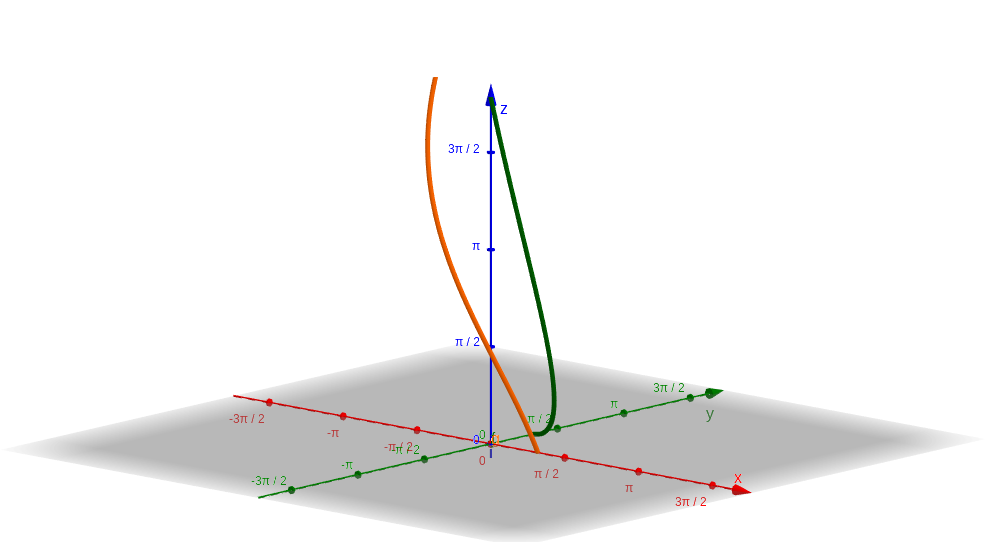
\includegraphics[width=0.45\textwidth]{img/Proyecto4_2.png}
	\caption{Claramente ambos vectores no son ortogonales, sólo en el origen}
\end{figure}
\noindent c) Encuentre la recta tangente a $\vec{\gamma}(t_0)$,  $t_0 = 4\pi$
\begin{definition}[Recta tangente]
	Si $ \vec{\gamma}(t) $ es una trayectoria en $ \R^3 $ (\textit{i.e. } $ \vec{\gamma} : \R \to \R^3 $) con $ \vec{\gamma}(t) \neq 0 \qquad \forall t \in \R$, entonces la ecuación de la recta tangente en $ t_0 $ es 
	\[  \l(t) = \vec{\gamma'}(t_0)(t-t_0) + \vec{\gamma}(t_0)  \]
\end{definition}
Por lo tanto 
\begin{align*}
	\l(t) &= (1,0,8\pi)(t - 4\pi) + (0,1,16\pi^2) && \text{Por el inciso a)}\\
	\l(t) &= (t - 4\pi,0,8\pi t - 32\pi^2) + (0,1,16\pi^2) && \text{Por distributividad}\\
	\l(t) &= (t - 4\pi,1,8\pi t - 32\pi^2 + 16\pi^2) && \text{Sumando de manera directa}\\
	\l(t) &= (t - 4\pi,1,8\pi( t -  2\pi)) && \text{Factorizando}
\end{align*}

\begin{figure}[h!]
	\centering
	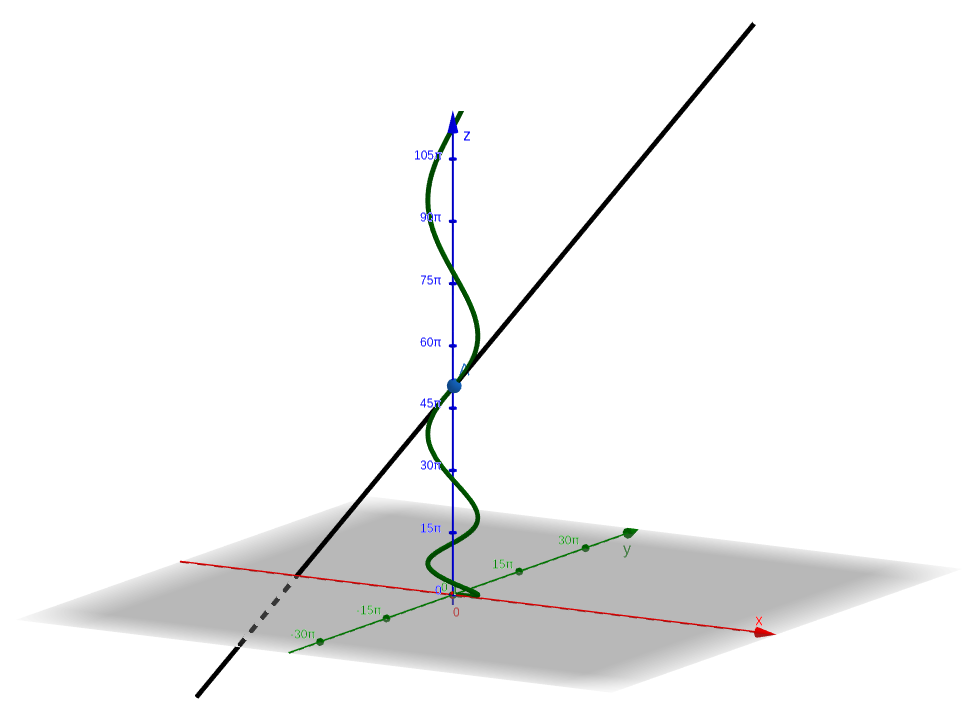
\includegraphics[width=0.3\textwidth]{img/Proyecto4_3.png}
	\caption{\small Ajustando los ejes un poco podemos apreciar que efectivamente se trata de la recta tangente }
\end{figure}


\newpage
\noindent d) ¿Dónde se intersecará esta línea con el plano $xy$?\\


Tomemos en cuenta $ \l(t) = (x(t), y(t), 0) $ entonces lo único que tenemos que resolver es 
\begin{align*}
	8\pi(t -2\pi) &= 0 && \text{Planteando la ecuación}\\
	t -2\pi &= 0 && \text{Multiplicando por el inverso multiplicativo de } 8\pi \\
	t &= 2\pi && \text{Añadiendo en ambos miembros } 2\pi \\
\end{align*}
es decir, hay que evaluar $ \l(t_0) $ en $ t_o = 2\pi $, esto es $ B = (-2\pi,1,0) $
\begin{figure}[h!]
	\centering
	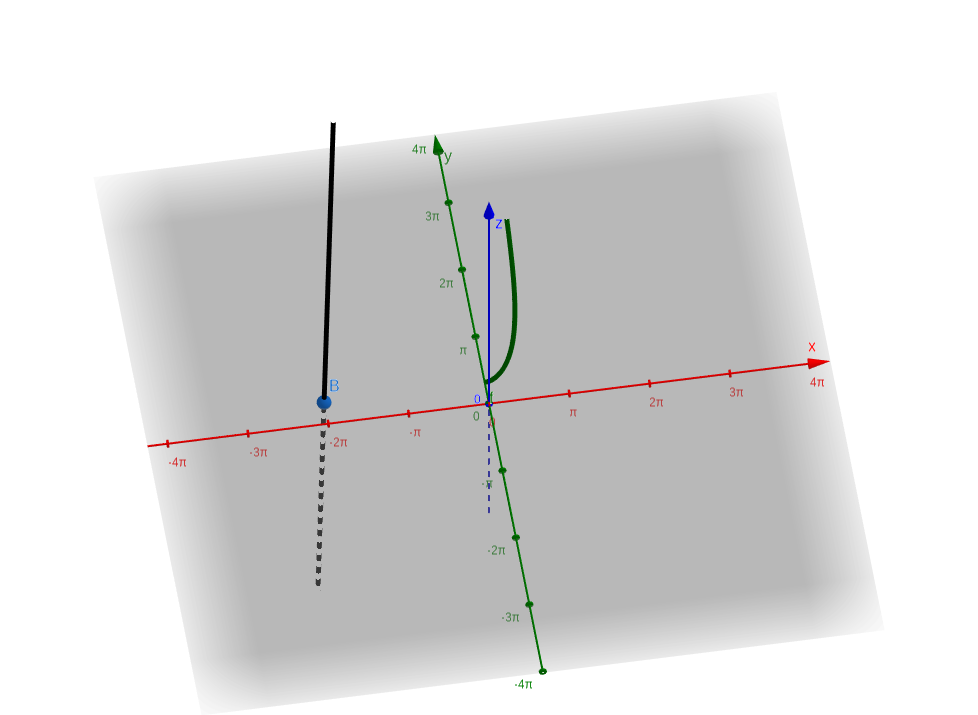
\includegraphics[width=0.7\textwidth]{img/Proyecto4_4.png}
	\caption{Se puede observar que efectivamente, la recta $ \l $ interseca al plano $ xy $ en B}
\end{figure}


\end{document}
